\documentclass{beamer}
\usepackage{beamerthemesplit} 
\usepackage[utf8]{inputenc}
\usepackage{default}
\usepackage{graphicx}
\usepackage{float}
\usepackage{color, colortbl}
\usepackage{xcolor}
\usepackage{caption}
\usepackage{subcaption}

\title{Localization Procedure}
	\subtitle{Orchestrating position estimation protocols in randomly deployed WSNs}
\author[Sanabria-Russo, L.]{Luis Sanabria-Russo, Cristina Cano, Boris Bellalta}
\institute[UPF]{Universitat Pompeu Fabra\\
				NeTS Research Group\\
				Barcelona, Spain}
\date{\today}



\begin{document}
%------------------Title Page---------------------%
\frame{\titlepage}

%\frame{\frametitle{Table of contents}\tableofcontents}

\section{Introduction}\label{intro}
\frame{\frametitle{What are Randomly Deployed WSNs?}
	\begin{itemize}
		\item Nodes are placed randomly over a field.
		\item It also encompasses deployments made at convenience (like home surveillance).
	\end{itemize}
	
	\begin{figure}[htbp]
		\centering
		\begin{subfigure}{.5\textwidth}
			\centering
			\includegraphics[width=0.6\linewidth, angle=-90]{figures/topology.eps}
			\caption{\tiny Example random deployment of nodes
			\label{fig:topology}}
			\end{subfigure}%
		\begin{subfigure}{.5\textwidth}
			\centering
			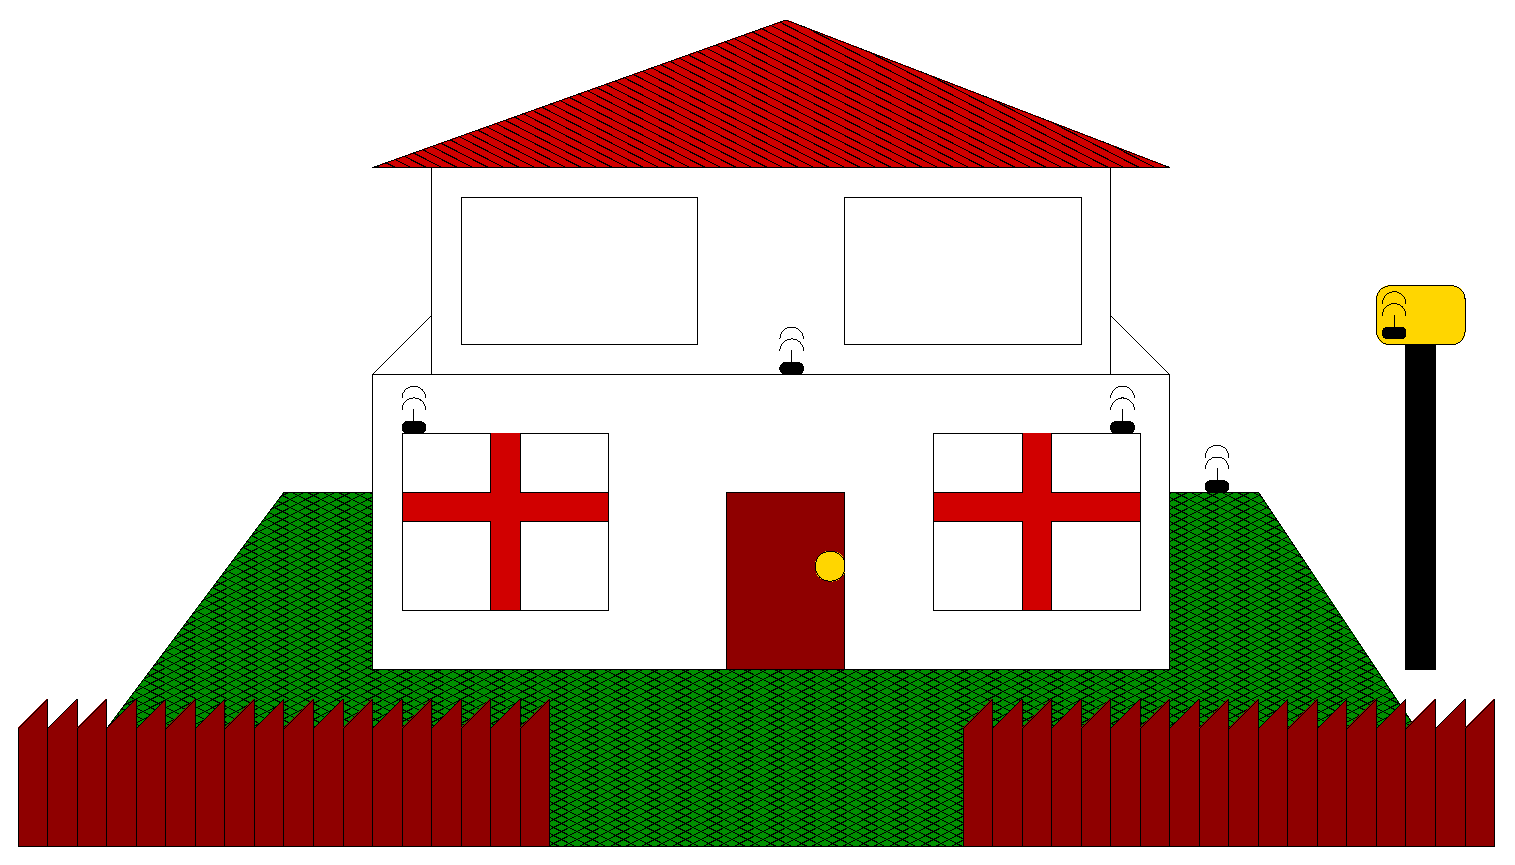
\includegraphics[width=\linewidth]{figures/house.eps}
			\caption{\tiny Example home surveillance deployment
			\label{fig:house}}
			\end{subfigure}
%	\caption{}
	\end{figure}

}

\end{document}
